\documentclass{article}

\usepackage{fontspec}
\usepackage{polyglossia}
\usepackage{notomath}
\setmainfont{GFS Artemisia}
\setsansfont{Source Code Pro}
\setmonofont{Source Code Pro}
\newfontfamily\greekfont[Script=Greek]{GFS Artemisia}
\newfontfamily\greekfontsf[Script=Greek]{GFS Artemisia}
\newfontfamily\greekfonttt[Script=Greek]{Source Code Pro}

%languages
\setdefaultlanguage{greek}
\setotherlanguages{english}


%typing
\usepackage{hyphenat}
\usepackage{float}
\usepackage{color, colortbl}
\usepackage{placeins}

%captions
\usepackage{caption}
\usepackage{subcaption}

%bib
% \usepackage{biblatex}
% \addbibresource{bib.bib}

%gemoetry
\usepackage[a4paper,top=1.2cm,bottom=1.2cm,left=1.2cm,right=1.2cm,marginparwidth=1.5cm]{geometry}

%images
\usepackage{graphicx}
\usepackage{tikz}

%ref
\usepackage[colorlinks=true, allcolors=blue]{hyperref}


\usepackage[export]{adjustbox}

%label
\usepackage{enumitem}
\renewcommand{\labelenumii}{\arabic{enumi}.\arabic{enumii}}
\renewcommand{\labelenumiii}{\arabic{enumi}.\arabic{enumii}.\arabic{enumiii}}
\renewcommand{\labelenumiv}{\arabic{enumi}.\arabic{enumii}.\arabic{enumiii}.\arabic{enumiv}}

%columnnew
\newcolumntype{g}{>{\columncolor{gray}}l}

%colors
\usepackage[dvipsnames]{xcolor}
\definecolor{gray}{gray}{0.9}
\definecolor{blue}{RGB}{82, 138, 174}
\definecolor{green}{RGB}{140, 219, 169}
\definecolor{yellow}{RGB}{253, 221, 92}

% \usepackage{titling}
% \setlength{\droptitle}{-20em}             %allagh glwssas
\hypersetup{
    colorlinks = true,
    linkcolor=black}


\usepackage{autobreak}


%Customize tables
\renewcommand{\arraystretch}{1.2}
% \rowcolors{2}{gray}{white}



\captionsetup[table]{
    format=plain,
    labelfont={small,it,bf}, % Small, italic, and bold label
    textfont={small,it}, % Italic text
    labelsep=colon % Colon separator
}



% Customize the figure caption
\captionsetup[figure]{
    format=plain,
    labelfont={small,it,bf}, % Small, italic, and bold label
    textfont={small,it}, % Italic text
    labelsep=colon % Colon separator
}

\makeatletter
\renewcommand*{\p@table}{\textit{Πίν. }}
\renewcommand*{\p@figure}{\textit{Σχ. }}
\renewcommand*{\p@equation}{\textit{Εξ. }}
\makeatother

\begin{document}
%TITLE
\newcommand{\uni}{ΑΡΙΣΤΟΤΕΛΕΙΟ ΠΑΝΕΠΙΣΤΗΜΙΟ ΘΕΣΣΑΛΟΝΙΚΗΣ}
\newcommand{\faculty}{ΠΟΛΥΤΕΧΝΙΚΗ ΣΧΟΛΗ}
\newcommand{\tmhma}{ΤΜΗΜΑ ΜΗΧΑΝΟΛΟΓΩΝ ΜΗΧΑΝΙΚΩΝ}


\newcommand{\titlos}{Δυναμικά φαινόμενα}
\newcommand{\ypotitlos}{Bonus Εργασία - Ειδικά Κεφάλαια Πεπερασμένων Στοιχείων}


\newcommand{\onomaauthor}{ΒΑΣΙΛΕΙΟΣ ΠΑΠΑΜΙΧΑΗΛ}


\newcommand{\advisor}{Γάκιας Χρήστος}
\newcommand{\mailauthor}{\href{mailto:vasilepi@meng.auth.gr}{vasilepi@meng.auth.gr}}
\newcommand{\aem}{6920}
\newcommand{\hmeromhnia}{\today}



\begin{titlepage}
    \begin{center}
    \raisebox{20mm}{
    \begin{tikzpicture}
        \draw (0,0) -- (6,0);
    \end{tikzpicture}}
\includegraphics[width=4cm]{media/autheng.jpg}\raisebox{20mm}{\begin{tikzpicture}
        \draw (0,0) -- (6,0);
    \end{tikzpicture}}
     \end{center}
    
    \begin{center}
        \large
        \uni\\
        \normalsize
        \faculty\\
        \vspace{1em}
        \tmhma
    \end{center}

    \vspace{2cm}
    \begin{center}
        \Large
        \textbf{\titlos}\\
        \vspace{1em}
        \large
        \textit{\ypotitlos}
    \end{center}
    \begin{center}
        \begin{tikzpicture}
        \draw (0,0) -- (4,0);
    \end{tikzpicture}\\
    \vspace{7em}
    \Large
    \textcolor{BrickRed}{\textbf{\onomaauthor}}\\
    \vspace{3em}
    
\includegraphics[width=0.3\textwidth]{media/newlogov3-cropped-content.png}
    \end{center}

    \vspace{7em}
    \hspace{4ex}
    \begin{minipage}[t]{0.45\textwidth} 
        \raggedright
        \textbf{Υπεύθυνος}: \advisor\\
        \textbf{Email}: \mailauthor\\
        \textbf{ΑΕΜ}: \aem
    \end{minipage}\\

    \vspace{4cm}
    \begin{center}
        \textit{\hmeromhnia}\\
        \begin{tikzpicture}
            \draw (0,0) -- (15,0);
        \end{tikzpicture}
    \end{center}
    
    
\end{titlepage}
\tableofcontents
%MAIN BODY

\section{Εισαγωγή}
\subsection{Παρουσίαση προβλήματος}

Στη παρόν εργασία μελετάται η ελαστοπλαστική συμπεριφορά υλικού τόσο σε κυκλική φόρτιση όσο και σε καθαρό εφελκυσμό. Σκοπός είναι, η αναπαργωγή των πειραματικών δεδομένων του υλικού και πιο συγκεκριμένα της καμπύλης τάσης παραμόρφωσης μονοτονικής συμπεριφοράς αλλά και των βρόγχων υστέρησης, δηλαδή της σταθεροποιημένης καμπύλης υλικού κυκλική συμπεριφοράς. Η όλη μελέτη γίνεται σε κύβο $10\times 10\times 10\; mm$ διαστάσεων που φορτίζεται εφελκυστικά. 
\par Η επιλογή του υλικού ήταν ανοιξείδωτος χάλυβας 316L σύμφωνα με την \cite{RASMUSSEN200347}. Στη συγκεκριμένη μελέτη δίνονται οι σταθερές κυκλικής συμπεριφοράς για διάφορα δοκίμια του υλικού. Παρακάτω φαίνονται οι σταθερές του υλικού που ακολουθούν το μοντέλο:
\begin{equation}
    \epsilon = \frac{\sigma}{E_0} + 0.002 \bigg(\frac{\sigma}{\sigma_{0.2}} \bigg)^n
\end{equation}
Τα δεδομένα που επιλέχθηκαν ήταν προφανώς μόνο για δοκίμια πάχους 10 χιλιοστών ενώ για τη μοντελοποίηση έπειτα χρησιμοποιήθηκαν οι average τιμές.
\begin{table}[H]
    \centering
    \rowcolors{2}{gray}{white}
        \begin{tabular}{|c|c|c|c|c|c|c|c|c|}
        \hline
        \rowcolor{Dandelion}
        Spec. \# & $t\; [mm]$ & l. rate & $\sigma_{0.2}\; [MPa]$ & $\sigma_{1.0}\; [MPa]$ & $\sigma_u\; [MPa]$ & elong \% & $E_0 \; [GPa]$ & n\\
        \hline
        LT1R & 10 & 3 & 252.8 & 296.3 & 585.7 & 50 & 185.5 & 7.9 \\
        \hline
        LT2R & 10 & 0.3 & 244.7 & 288.6 & 586.5 & 47 & 187.8 & 7.9 \\
        \hline
        LT3R & 10 & 30 & 265.1 & 307.4 & 584.8 & 52 & 195.4 & 5.8 \\
        \hline
        LT4R & 10 & 3 & 262.6 & 303.6 & 588.1 & 48 & 194.6 & 7.5 \\
        \hline
        LT5R & 10 & 0.3 & 248.1 & 291.1 & 590.3 & 49 & 189.4 & 9.8 \\
        \hline
        LT6R & 10 & 30 & 295.6 & 319.7 & 588.9 & 48 & 200.1 & 6.7 \\
        \hline
        LT7R & 10 & 3 & 260.6 & 295.3 & 579.5 & 52 & 196.9 & 8.8 \\
        \hline
        Average & 10 & - & 272.5 & 311.3 & 583.9 & 47.9 & 192.8 & 7.1 \\
        \hline
        \end{tabular}
    \caption{Πειραματικά αποτελέσματα 316L υπό εφελκυστική φόρτιση.}
    \label{tab:peiram}
\end{table}
Ζητούνται πιο συγκεκριμένα:

\begin{itemize}
\item Θα δημιουργήσετε έναν κύβο διαστάσεων 10x10x10 mm και θα τον
διακριτοποιήσετε με τουλάχιστον 3 στοιχεία σε κάθε διαστασή του.
\item Θα εφαρμόσετε κατάλληλες οριακές συνθήκες ώστε να φορτίζεται σε καθαρό
εφελκυσμό.
\item Υπό εφελκυστική φόρτιση, θα εξεταστεί η ελαστοπλαστική συμπεριφορά,
ακολουθώντας τις εξής παραδοχές:
\begin{itemize}
\item Τέλεια πλαστική συμπεριφορά
\item Γραμμική κράτυνση
\item Εκθετική κράτυνση (δημιουργώντας καμπύλη με πολλά σημεία)
\end{itemize}
Θα πρέπει να αναπαράγετε με τη μέγιστη δυνατή ακρίβεια για κάθε παραδοχή, τα
δεδομένα του υλικού που έχετε επιλέξει. Επίσης, θα πρέπει να εξετάσετε τις
παραμέτρους προεκβολής που δίνει ως επιλογή ο επιλυτής.
\item Υπό εναλλασσόμενη φόρτιση θα εξετάσετε την σταθεροποιημένη κυκλική
συμπεριφορά του υλικού, ακολουθώντας της εξής παραδοχές:
\begin{itemize}
\item Ισοτροπική κράτυνση, σε συνδυασμό με τις παραδοχές ελαστοπλαστικής
συμπεριφοράς του ερωτήματος 3.
\item Κινηματική κράτυνση, σε συνδυασμό με τις παραδοχές ελαστοπλαστική
συμπεριφοράς του ερωτήματος 3.
\item Η κυκλική συμπεριφορά θα πρέπει να εξεταστεί στην περίπτωση ελέγχου
δύναμης και ελέγχου μετατόπισης.
\end{itemize}
Θα πρέπει να αναπαράγετε με τη μέγιστη δυνατή ακρίβεια για κάθε παραδοχή, τα
δεδομένα του υλικού σε κυκλική φόρτιση που έχετε επιλέξει.
\item Να εξετάσετε παραμέτρους του επιλυτή που αφορούν την αστοχία του υλικού σε
κάποια μέγιστη τιμή τάσης ή/και παραμόρφωσης.
\item Θα πρέπει να είστε σε θέση να ποσοτικοποιήσετε τις αποκλίσεις που θα
παρατηρήσετε καθώς και να τις εξηγήσετε κατάλληλα.
\item Οποιοδήποτε φαινόμενο παρατηρήσετε στα αποτελέσματά σας, θα πρέπει να το
χαρακτηρίσετε και να το εξηγήσετε με τις κατάλληλες βιβλιογραφικές αναφορές.
\item Είστε ελεύθεροι να χρησιμοποιήσετε οποιαδήποτε άλλη παράμετρο προσφέρει ο
επιλυτής.
\end{itemize}

Σχετικά με τα διαφορετικά πλαστικά μοντέλα, αυτό που αναμένεται από την επίλυση, είναι κανένα από αυτά να μην προσεγγίσει τέλεια τη κυκλική συμπεριφορά του υλικού. Όσο αναφορά τη μονοτονική καμπύλη, η γραμμική κράτυνση παραμορφώνει πλαστικά το υλικό ακολουθώντας γραμμική καμπύλη, η τέλεια πλαστική διατηρεί την ίδια τάση με αυξανόμενη παραμόρφωση, ενώ η εκθετική κράτυνση ακολουθεί τη καμπύλη Ramberg-Osgood. Όπως παρατηρείται και από το \ref{fig:hard}, τα διαφορετικά ήδη πλαστικότητας εμφανίζουν αρκετά διαφορετική δυναμική συμπεριφορά. Το μοντέλο που προσεγγίζει καλύτερα όπως φαίνεται τη τυπική συμπεριφορά των βρόγχων υστέρησης είναι η μίξη της κινηματική και της ισοτροπικής κράτυνσης.
\begin{figure}[H]
    \centering
    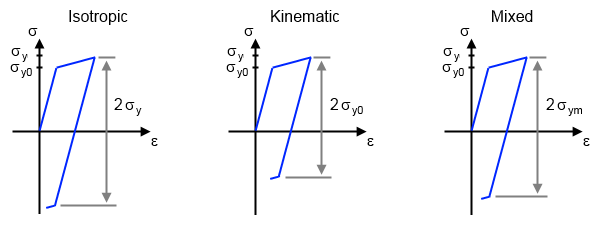
\includegraphics[width=0.6\linewidth]{media/hard.png}
    \caption{Μοντέλα πλαστικότητας υπό κυκλική εναλλασόμενη φόρτιση.}
    \label{fig:hard}
\end{figure} 

\section{Μοντελοποίηση}

\subsection{Μονοτονική συμπεριφορά}
Όσο αναφορά τη μονοτονική συμπεριφορά, δημιουργείται κύβος με 5 στοιχεία σε κάθε ακμή. Για τις οριακές συνθήκες, ώστε νε επιτευχθεί καθαρός εφελκυσμός, η μια πλευρά του κύβου περιορίζεται στον άξονα εφαρμογής της δύναμης, στο ίδιο επίπεδο που βρίσκεται αυτή η επιφάνεια περιορίζονται δύο ακμές του κύβου στους άλλους δύο άξονες (με τις ακμές να είναι κάθετες στον άξονα στον οποίο περιορίζονται). Γίνεται πιο εύκολα αντιληπτό και από το \ref{fig:bcs}. Οι ίδιες οριακές συνθήκες χρησιμοποιήθηκαν προφανώς και για τη θράυση αλλά και για τη κυκλική φόρτιση.

\begin{figure}[H]
    \centering
    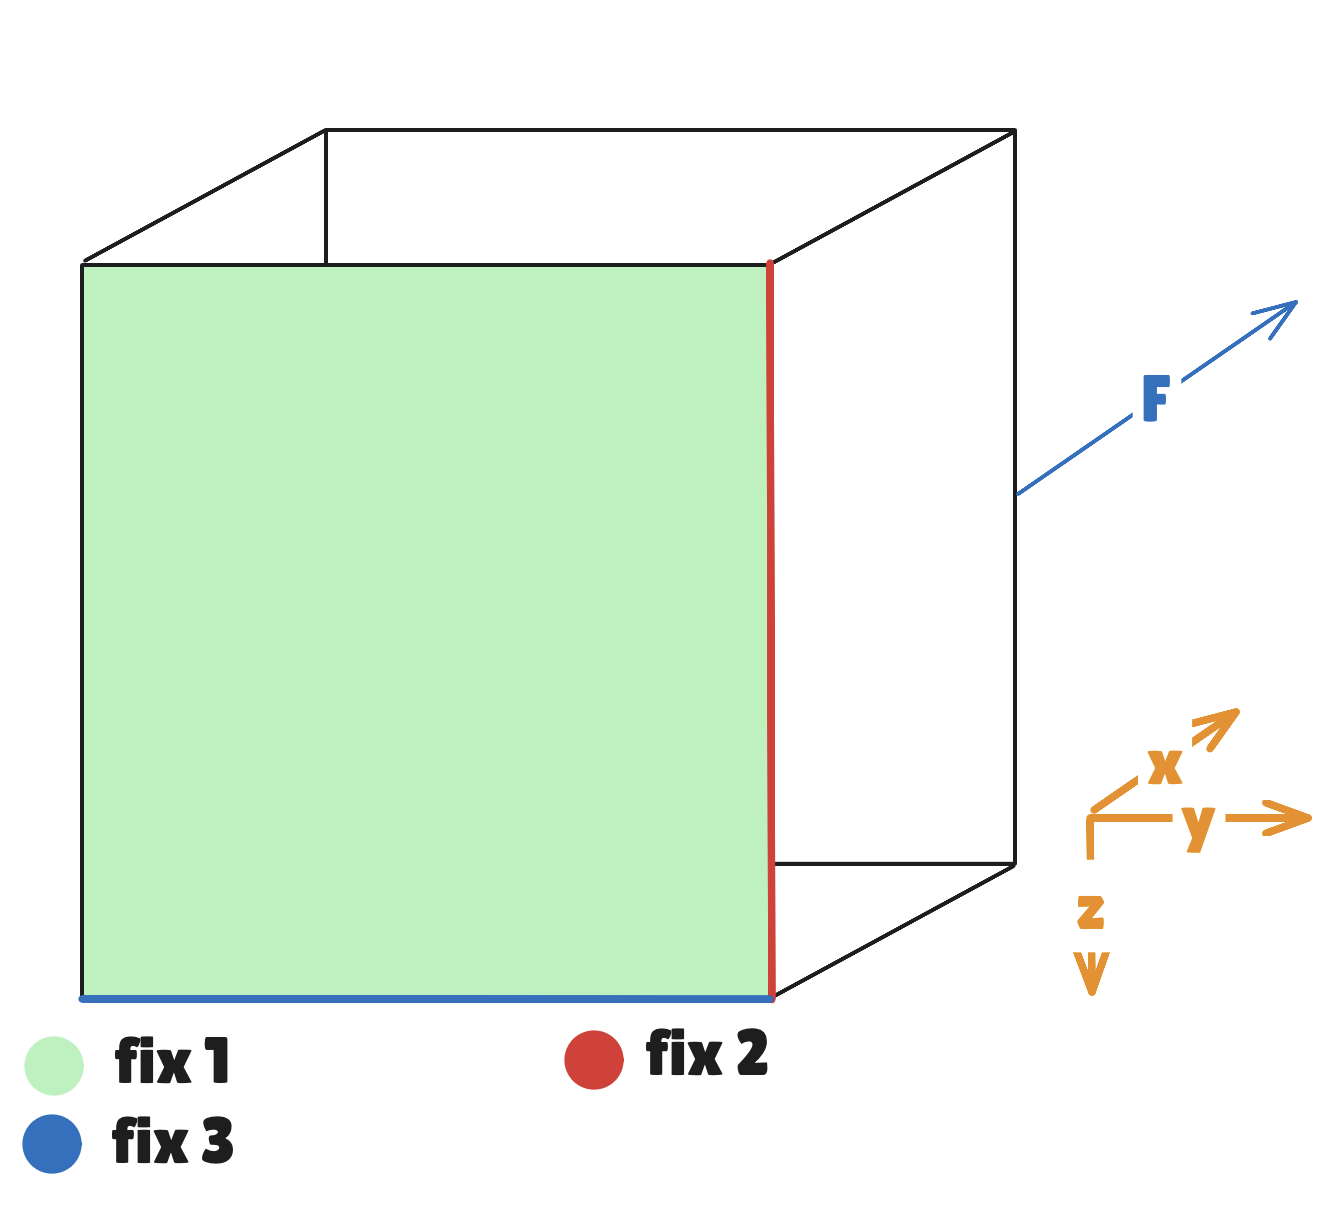
\includegraphics[width=0.4\linewidth]{media/bcs.png}
    \caption{Οριακές συνθήκες για επίτευξη καθαρού εφελκυσμού κύβου.}
    \label{fig:bcs}
\end{figure}

Επίσης, για μεγαλύτερη σταθερότητα κατά την επίλυση, χρησιμοποιήθηκε μετατόπιση και όχι φορτίο ώστε να επιτευχθεί η παραμόρφωση του κύβου. Η μετατόπιση που πρέπει να δωθεί στην επιφάνεια του κύβου είναι προφανώς $u = \epsilon_{max} \cdot 10$, ώστε να φτάσει το υλικό αυτή τη παραμόρφωση που εμφανίζεται και στην Ramberg-Osgood. Η μέγιστη παραμόρφωση  υπολογίζεται από την Ramberg-Osgood αναλυτικά έως την τάση $\sigma_u$ του υλικού, δηλαδή $\epsilon_{max} = \epsilon_u$. 
\par Για τον ορισμό της πλαστικότητας του υλικού ορίζονται πίνακες πλαστικότητας σύμφωνα με τις προδιαγραφές του επιλυτή. Παρακάτω φαίνονται τα αναλυτικά αποτελέσματα καθώς και μόνο η πλαστική παραμόρφωση του υλικού, δηλαδή οι τιμές εισαγωγής στον επιλυτή.
\begin{figure}[H]
    \centering
    \begin{subfigure}{0.45\linewidth}
        \centering
        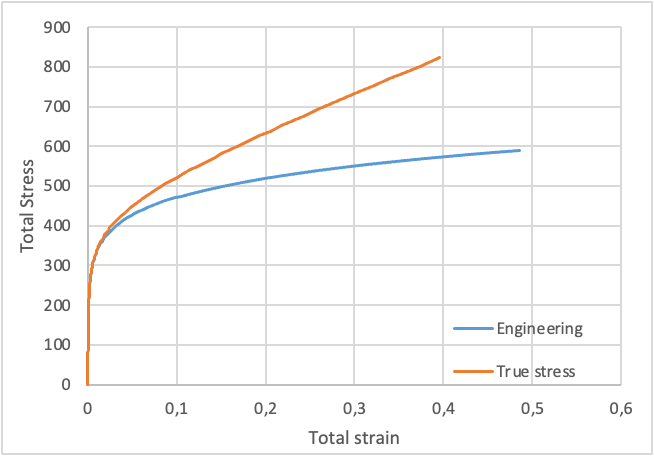
\includegraphics[width=\linewidth]{media/ragood.png}
        \caption{Αναλυτική καμπύλη Ramberg-Osgood 316L.}
        % \label{fig:label1}
    \end{subfigure}
    \hfill
    \begin{subfigure}{0.45\linewidth}
        \centering
        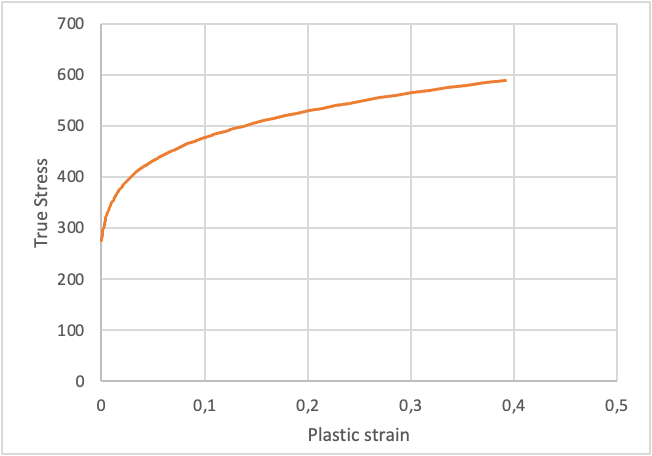
\includegraphics[width=\linewidth]{media/plabaqus.png}
        \caption{Πλαστική παραμόρφωση 316L.}
        % \label{fig:label2}
    \end{subfigure}
    \caption{Αναλυτικές καμπύλες μονοτωνικής συμπεριφοράς ανοιξείδωτου χάλυβα 316L.}
    \label{fig:anal}
\end{figure}
Για τις επιλύσεις τέλειας πλαστικότητας και γραμμικής πλαστικότητας δίνονται μόνο το πρώτο σημείο της καμπύλης πλαστικής παραμόρφωσης και το πρώτο και τελευταίο σημείο της καμπλύλης αντίστοιχα. 
\par Όσο αναφορά την κατάστρωση της επίλυσης, είναι πολύ σημαντική η επιλογή του βήματος επίλυσης. Στην αρχή η επίλυση έγινε με \texttt{TIME INC} = 0.1 και αποδείχθηκε, ότι δεν προσαρμόζεται σωστά η αριθμητική καμπύλη στο μέτρο ελαστικότητας του υλικού. Έτσι, το μοντέλο επιλύεται δεύτερη φορά με μικρότερο βήμα.
\begin{figure}[H]
    \centering
    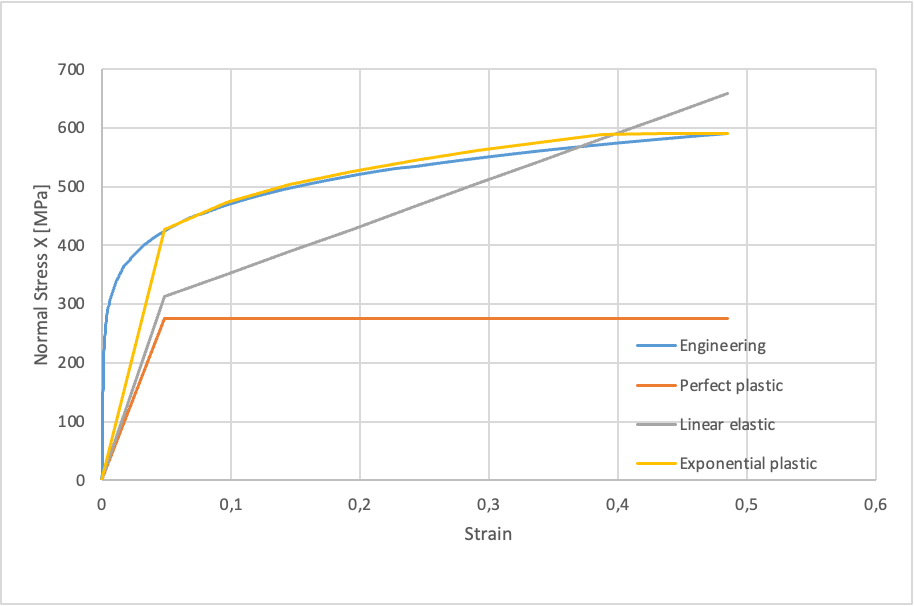
\includegraphics[width=0.8\linewidth]{media/static-false.png}
    \caption{Μη καλή προσέγγιση μονοτονικής συμπερφοράς λόγω μεγάλου βήματος επίλυσης.}
    \label{fig:statfalse}
\end{figure}

\subsection{Κυκλική συμπεριφορά}
Για την επίλυση της κυκλικής φόρτισης, γίνεται πιο πυκνό πλέγμα με 8 στοιχεία σε κάθε ακμή ώστε να επιτευχθεί πιο σταθερή λύση. Εδώ, το πλάτος μετατόπισης αλλάζει ώστε να επιτευχθεί η κυκλική φόρτιση. Για την αναλυτική προσέγγιση χρησιμοποιούνται οι κυκλικές σταθερές από τη πηγή για τη δημιουργία του βρόγχου υστέρησης του υλικού. Ακολουθώντας τα διαφορετικά μοντέλα πλαστικότητας, αναμένεται η επιστροφή από τη μέγιστη μετατόπιση στην ελάχιστη να έχει διαφορετική τιμή εύρους τάσης με $\sigma_y = \sigma_{0.2}$. 
\par Είναι σημαντικό στην κυκλική φόρτιση, να δωθεί σωστός πίνακας πλαστικότητας. Στην ισοτρποική πλαστικότητα για παράδειγμα θα πρέπει να δωθεί εκτεταμένος πίνακας, με περισσότερες τιμές και όχι έως το όριο $\sigma_{0.2}$, καθώς τόσο κατά την αποφόρτιση όσο και κατά την επαναφόρτιση, το ισοτροπικό μοντέλο φτάνει όλο και πιο ψηλά με κάθε κύκλο φόρτισης. Σε λανθασμένη επίλυση με το συγκεκριμένο μοντέλο, δώθηκε μη εκτεταμένος πίνακας και το υλικό ανταποκρινόταν σε συνθήκες τέλειας πλαστικότητας από τη στιγμή που ξεπερνιόταν το όριο τάσης του πίνακα πλαστικότητας. Αυτό γίνεται εμφανές και παρακάτω, όπου μόλις η τάση φτάνει στο όριο του πίνακα πλαστικότητας $\sigma_{0.2}$, το υλικό φέρεται σαν τέλεια πλαστικό.
\begin{figure}[H]
    \centering
    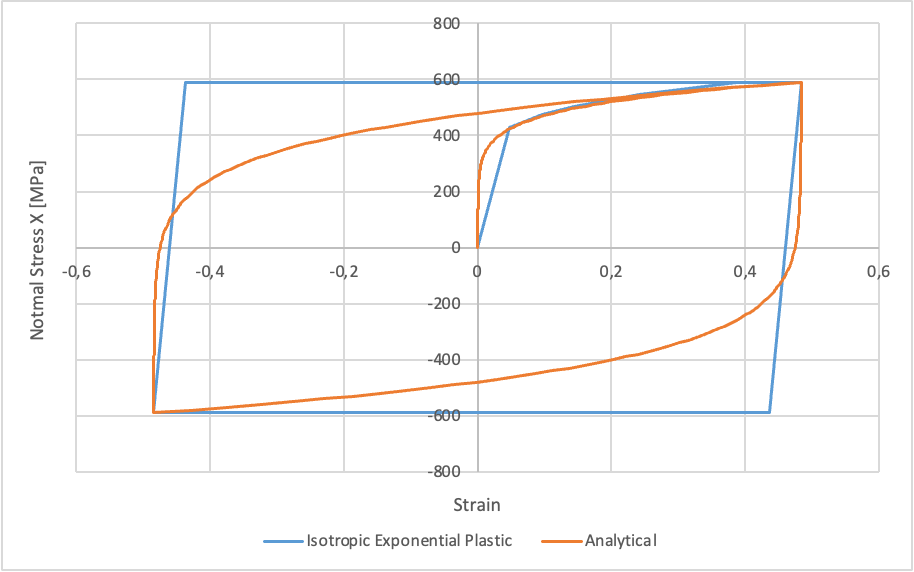
\includegraphics[width=0.8\linewidth]{media/dynamic-false.png}
    \caption{Λανθασμένη επίλυση με μη εκτεταμένο πίνακα πλαστικότητας και ισοτροπικό μοντέλο.}
    \label{fig:dfalse}
\end{figure}

\subsection{Θραύση}
Σχετικά με τη θραύση, αναζητώνται παράμετροι του επιλυτή. Ο επιλυτής προσφέρει διάφορες δυνατότητες σχετικά με αναλύσεις που αφορούν τη θραύση του υλικού. Εδώ θα εξεταστεί η εξέλιξη της θράυσης και η διαγραφή στοιχείων που αστοχούν. Μετά το όριο $\sigma_u$ και εφόσον συνεχίζει να αυξάνεται η φόρτιση, η στιβαρότητα του υλικού τείνει να φθήνει έως ότου επέλθει η θραύση. Ρυθμίζοντας κατάλληλες παραμέτρους στον επιλυτή, μπορεί να συνυπολογίζεται το damage του υλικού καθώς αυξάνει η δύναμη φόρτισης, να ορισθεί ένα όριο μέγιστης υποβάθμισης (\texttt{MAX DEGRADATION}) του υλικού μετά από το οποίο θα επέλθει η θραύση, αλλά και πως θα συνεχίσει η καμπύλη τάσης παραμόρφωσης μετά από το όριο $\sigma_u$.
\par Οι παράμετροι αυτοί είναι οι παράμετροι εκκίνησης βλάβης και εξέλιξης της (\texttt{DAMAGE INITIATION}, \texttt{DAMAGE EVOLUTION}). Ο επιλυτής αναφέρει ότι η εκκίνηση της βλάβης εξαρτάται από το μοντέλο που θα επιλεγεί για την εκκίνηση. Εδώ επιλέγεται το κριτήριο ολκιμότητας (\texttt{DUCTILE CRITERION}), σύμφωνα με το οποίο η πλαστική παραμόρφωση στην έναρξη της βλάβης εξαρτάται από την τριαξονικότητα (triaxiality) και τον ρυθμό παραμόρφωσης (strain rate). Όσο αναφορά το triaxiality αυτό ορίζεται ως:
\begin{equation}
    \eta = -\frac{p}{q}
\end{equation}

Όπου, $p$ είναι η πίεση λόγω της τάσης και $q$ η ισοδύναμη Von-Mises τάση. Στην \cite{triaxiality} δίνεται από πειραματικά δεδομένα η υπολογισμένη triaxiality και αντίστοιχη τάση εκκίνησης της βλάβης για διάφορους ρυθμούς παραμόρφωσης. Έτσι, επιλέγοντας έναν συγκεκριμένο ρυθμό παραμόρφωσης και μια συγκεκριμένη τιμή triaxiality μπορεί να υπολογιστεί από το \ref{fig:triaxial} η παραμόρφωση στην οποία εμφανίζεται για πρώτη φορά η βλάβη.
\begin{figure}[H]
    \centering
    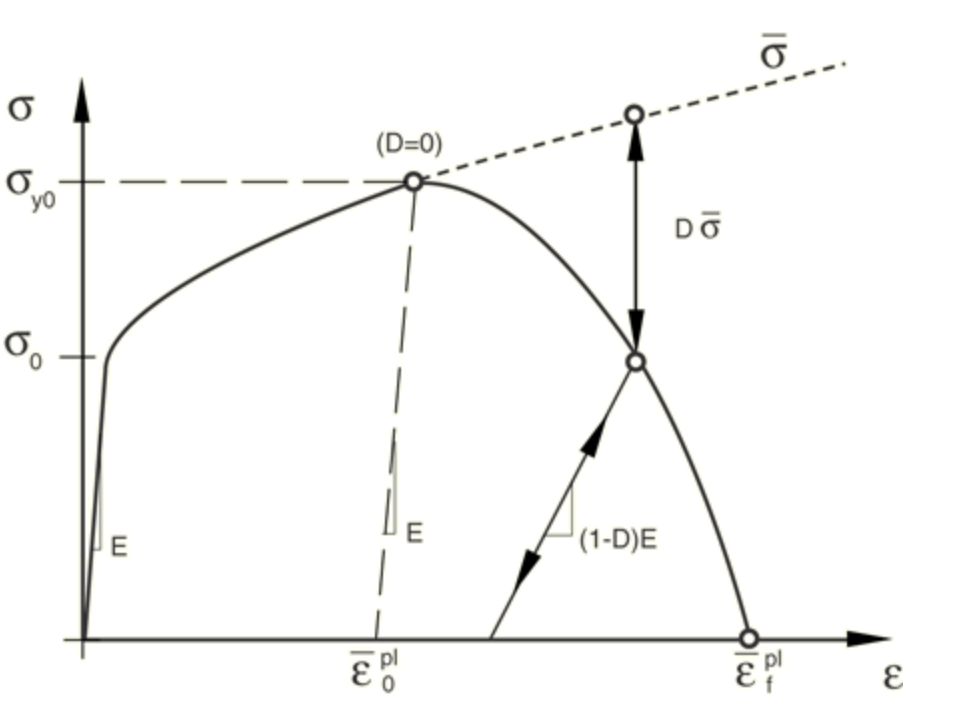
\includegraphics[width=0.6\linewidth]{media/abaqDE.png}
    \caption{Εξέλιξη βλάβης έως θράυση υλικού όπως αναγράφεται στο εγχειρίδιο του ABAQUS.}
    \label{fig:abaqDE}
\end{figure}

\begin{figure}[H]
    \centering
    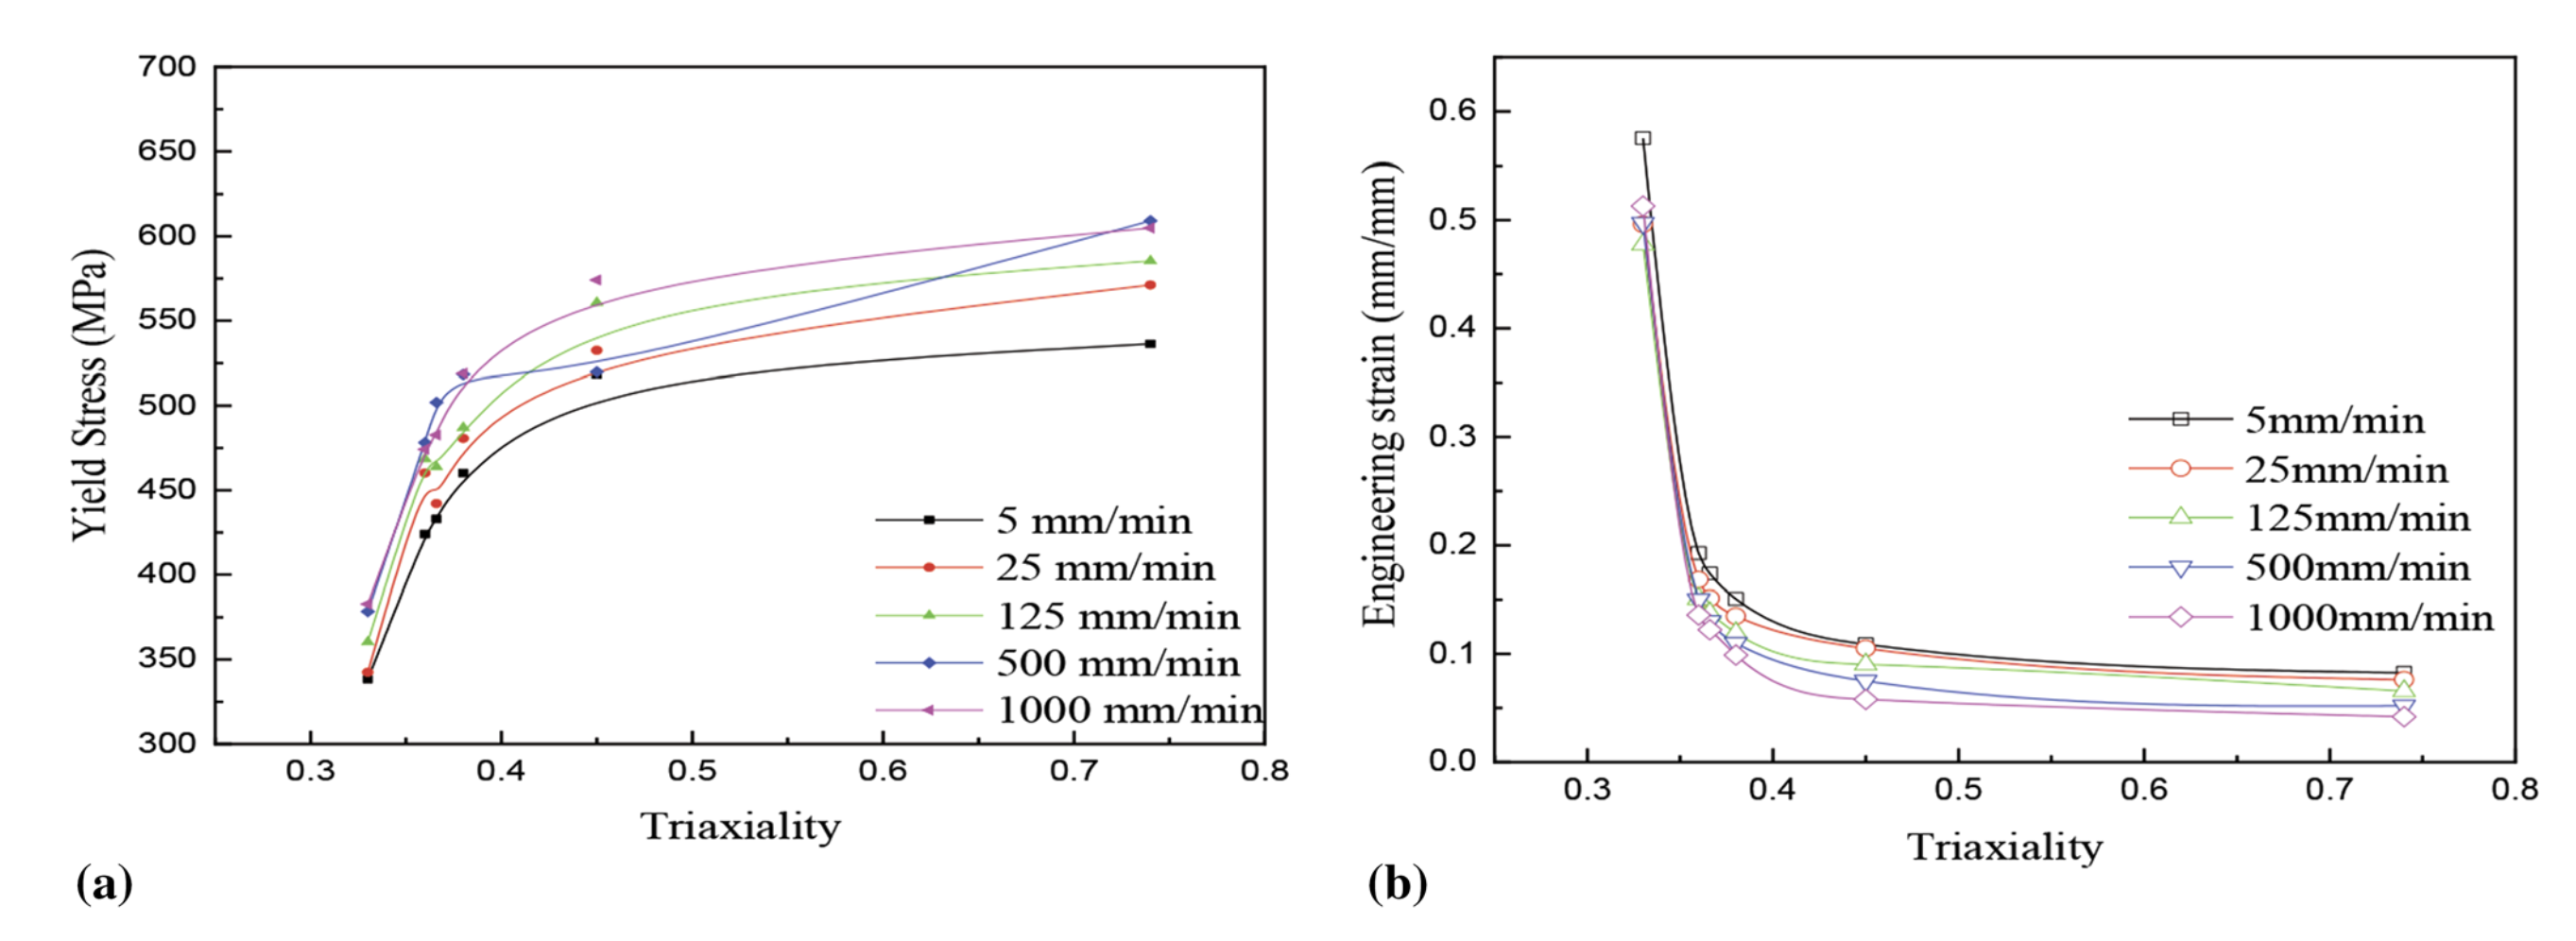
\includegraphics[width=0.9\linewidth]{media/triaxiCurve.png}
    \caption{Triaxiality για διάφορους ρυθμούς παραμόρφωσης για ανοξείδωτο χάλυβα 316L σύμφωνα με την \cite{triaxiality}.}
    \label{fig:triaxial}
\end{figure}


Όσο αναφορά την εξέλιξη της βλάβης, πρέπει να ορισθεί το μοντέλο χαλάρωσης (\texttt{SOFTENING}). Επιλέγοντας γραμμικό μοντέλο, σημαίνει ότι η παραμόρφωση μειώνεται γραμμικά έως ότου επέλθει η θραύση. Στο γραμμικό μοντέλο αρκεί να δοθεί σαν παράμετρος η ισοδύναμη μετατόπιση η οποία φτάνει το υλικό όταν επέρχεται θραύση. Η ισοδύναμη μετατόπιση είναι σύμφωνα με το \ref{fig:abaqDE}:
\begin{equation}
    u_{eq} = L\cdot (\overline{\epsilon}^{pl}_f - \overline{\epsilon}^{pl}_0)
\end{equation}
Όπου, $L$ είναι το χαρακτηριστικό μήκος του στοιχείου το οποίο είναι $\frac{10}{8}$, το οποίο θεωρείται μονάδα για λόγους ευκολίας. Εν τέλει, με το γραμμικό μοντέλο μετατόπισης όταν η βλάβη γίνει ίση με τη μονάδα, η μετατόπιση του υλικού φτάνει στη τιμή $u_{eq}$. Στην \cite{fracture} δίνεται η πλήρης καμπύλη τάσης παραμόρφωσης έως τη θράυση για το υλικό της παρόν εργασίας. Δυστυχώς, δεν βρέθηκαν δεδομένα για το ρυθμό παραμόρφωσης της εν λόγω καμπύλης και εν γένει δεν βρέθηκαν δεδομένα για το υλικό που συνδυάζουν όλους τις παραμέτρους που ζητούνται από τον επιλυτή για τη μελέτη της θραύσης σε μία δημοσίευση. Τελικά, η συγκεκριμένη ανάλυση στον επιλυτή δεν μπορεί να συγκριθεί με κάποιο πείραμα καθώς δεν μπορούσαν να βρεθούν δεδομένα αλλά γίνεται πιο πολύ για χάρην της εξερεύνησης των παραμέτρων που προσφέρει ο ABAQUS.
\begin{figure}[H]
    \centering
    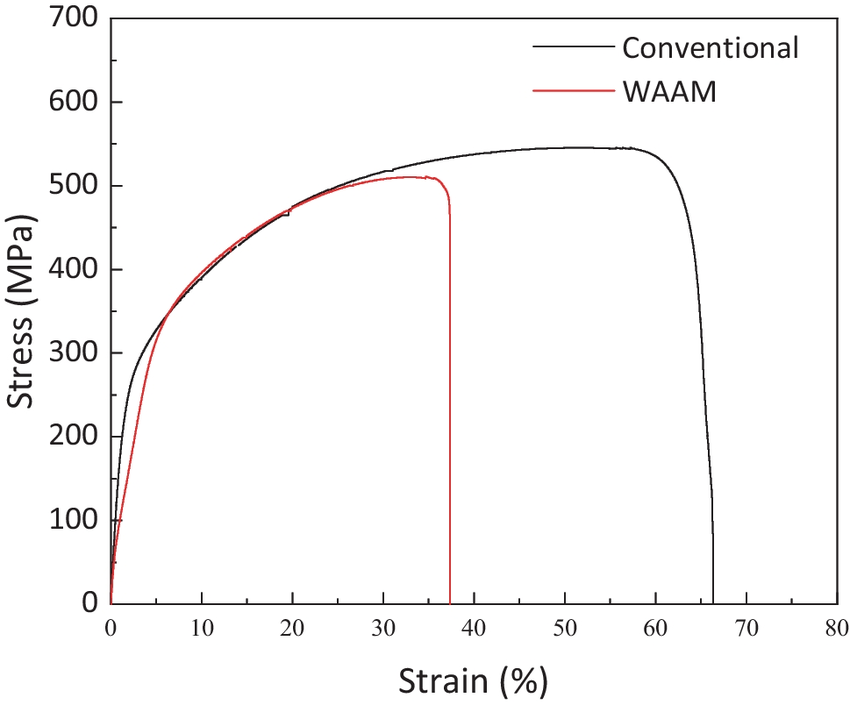
\includegraphics[width=0.6\linewidth]{media/fractureCurve.png}
    \caption{Εξέλιξη θραύσης για ανοξείδωτο χάλυβα 316L σύμφωνα με την \cite{fracture}.}
    \label{fig:fra}
\end{figure}
\par Επομένως, όσο αναφορά την θραύση, θα πρέπει να οριστεί τόσο η εξέλιξη της βλάβης όσο και η εκκίνηση στον επιλυτή. Επίσης, θα πρέπει να γίνει και επεξεργασία στο \texttt{SECTION} ώστε να είναι δυνατή η διαγραφή των στοιχείων. Εκεί ορίζεται και η μέγιστη βλάβη έπειτα από την οποία διαγράφονται τα στοιχεία. Οι παράμετροι που ορίστηκαν φαίνονται παρακάτω καθώς επιλέχθηκαν για ρυθμό παραμόρφωσης $5\; mm/min = 0.0833\; mm/s$, τριαξονικότητα ίση με $0.35$. Επίσης από το \ref{fig:fra} φαίνεται ισοδύναμη μετατόπιση περίπου ίση με $0.16$, συνυπολογίζοντας και το μήκος στοιχείου. Τα παρακάτω σημεία πρέπει επίσης να μπουν στο κώδικα του inp.

\begin{table}[H]
    \centering
    \rowcolors{2}{gray}{white}
        \begin{tabular}{|c|c|}
        \hline
        \rowcolor{Dandelion}
        Παράμετρος & Τιμή\\
        \hline
        Triaxiality & 0.35\\
        \hline
        Str.Rate & 0.0833\\
        \hline
        Eq.Pl.Strain & 0.58\\
        \hline
        uf.Pl & 0.16\\
        \hline
        MAX DEGRADATION & 0.99\\
        \hline
        \end{tabular}
    \caption{Παράμετροι επιλυτή για μελέτη θραύσης υλικού.}
    \label{tab:tablabel}
\end{table}


\begin{lstlisting}
** DAMAGE INITIATION
*DAMAGE INITIATION, CRITERION=DUCTILE
                     0.58,                     0.35,                   0.0833
*DAMAGE EVOLUTION, TYPE=DISPLACEMENT, SOFTENING=LINEAR
                     0.16,
**
\end{lstlisting}


\begin{lstlisting}
*SOLID SECTION, ELSET=P3;Default PSOLID Property, MATERIAL=M3;Default MATERIAL, CONTROLS=C1;Default SECTION CONTROLS
**

...

** SECTION CONTROLS
*SECTION CONTROLS, NAME=C1;Default SECTION CONTROLS, ELEMENT DELETION=YES, MAX DEGRADATION=0.99
\end{lstlisting}

\section{Αποτελέσματα Και Συζήτηση}
\subsection{Αποτελέσματα}
Παρακάτω παρατίθονται τα αποτελέσματα της εργασίας. Όσο αναφορά τη θράυση, μπορεί να παρατηρηθεί στο \ref{fig:steps} τρία διαδοχικά βήματα της επίλυσης. Φαίνεται η συσσώρευση βλάβης στην κλίμακα, ενώ η τρίτη εικόνα παρουσιάζεται κενή καθώς σε εκείνο το "χρονικό" βήμα τα στοιχεία ξεπεράσαν το όριο υποβάθμισης και διαγράφθηκαν. Δίνεται επίσης και το πως μεταβάλεται η βλάβη καθώς αυξάνεται η μετατόπιση του υλικού.
\begin{figure}[H]
    \centering
    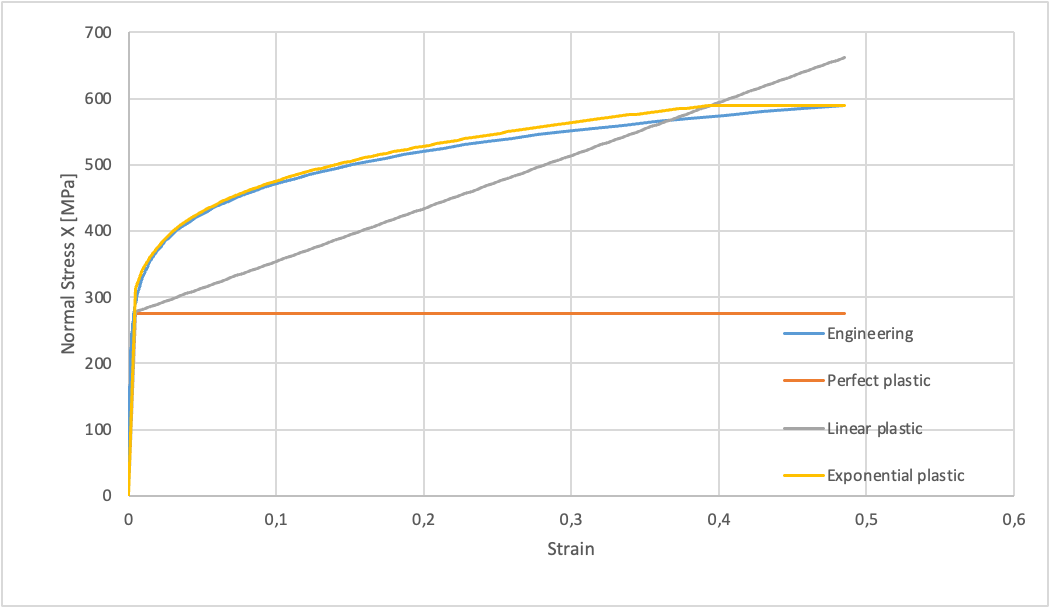
\includegraphics[width=0.7\linewidth]{media/static.png}
    \caption{Επίλυση μονοτωνικής συμπεριφοράς.}
    \label{fig:static}
\end{figure}

\begin{figure}[H]
    \centering
    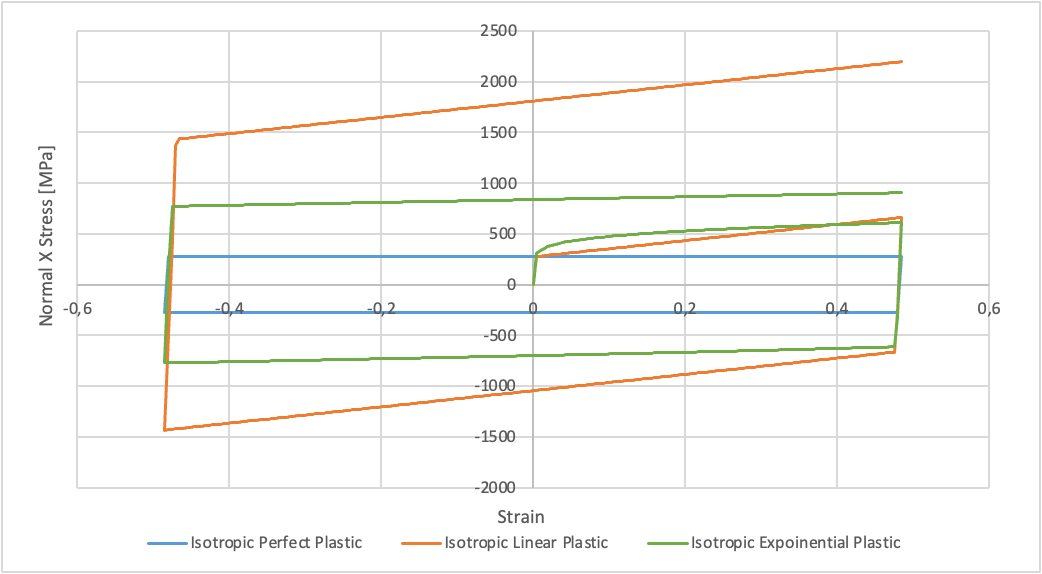
\includegraphics[width=0.7\linewidth]{media/dynamic-iso.png}
    \caption{Σύγκριση μοντέλων με ισοτροπική κράτυνση και διαφορετικά μοντέλα πλαστικότητας υπό κυκλική φόρτιση.}
    \label{fig:dyniso}
\end{figure}

\begin{figure}[H]
    \centering
    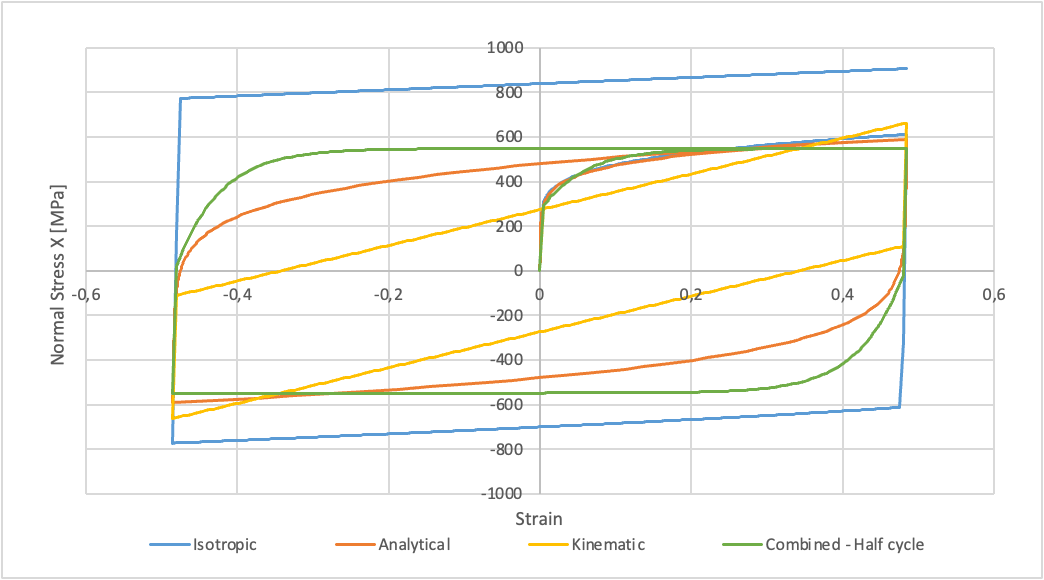
\includegraphics[width=0.7\linewidth]{media/dynamic.png}
    \caption{Επίλυση κυκλικής συμπεριφοράς.}
    \label{fig:dyn}
\end{figure}

\begin{figure}[H]
    \centering
    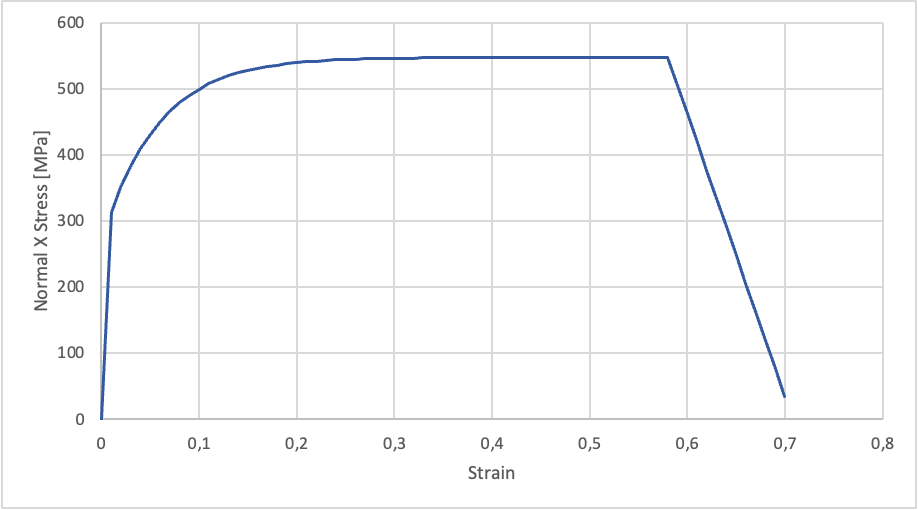
\includegraphics[width=0.7\linewidth]{media/fracture.png}
    \caption{Επίλυση εξέλιξης θράυσης υλικού.}
    \label{fig:fracture}
\end{figure}


\begin{figure}[H]
    \centering
    \begin{subfigure}{0.3\linewidth}
        \centering
        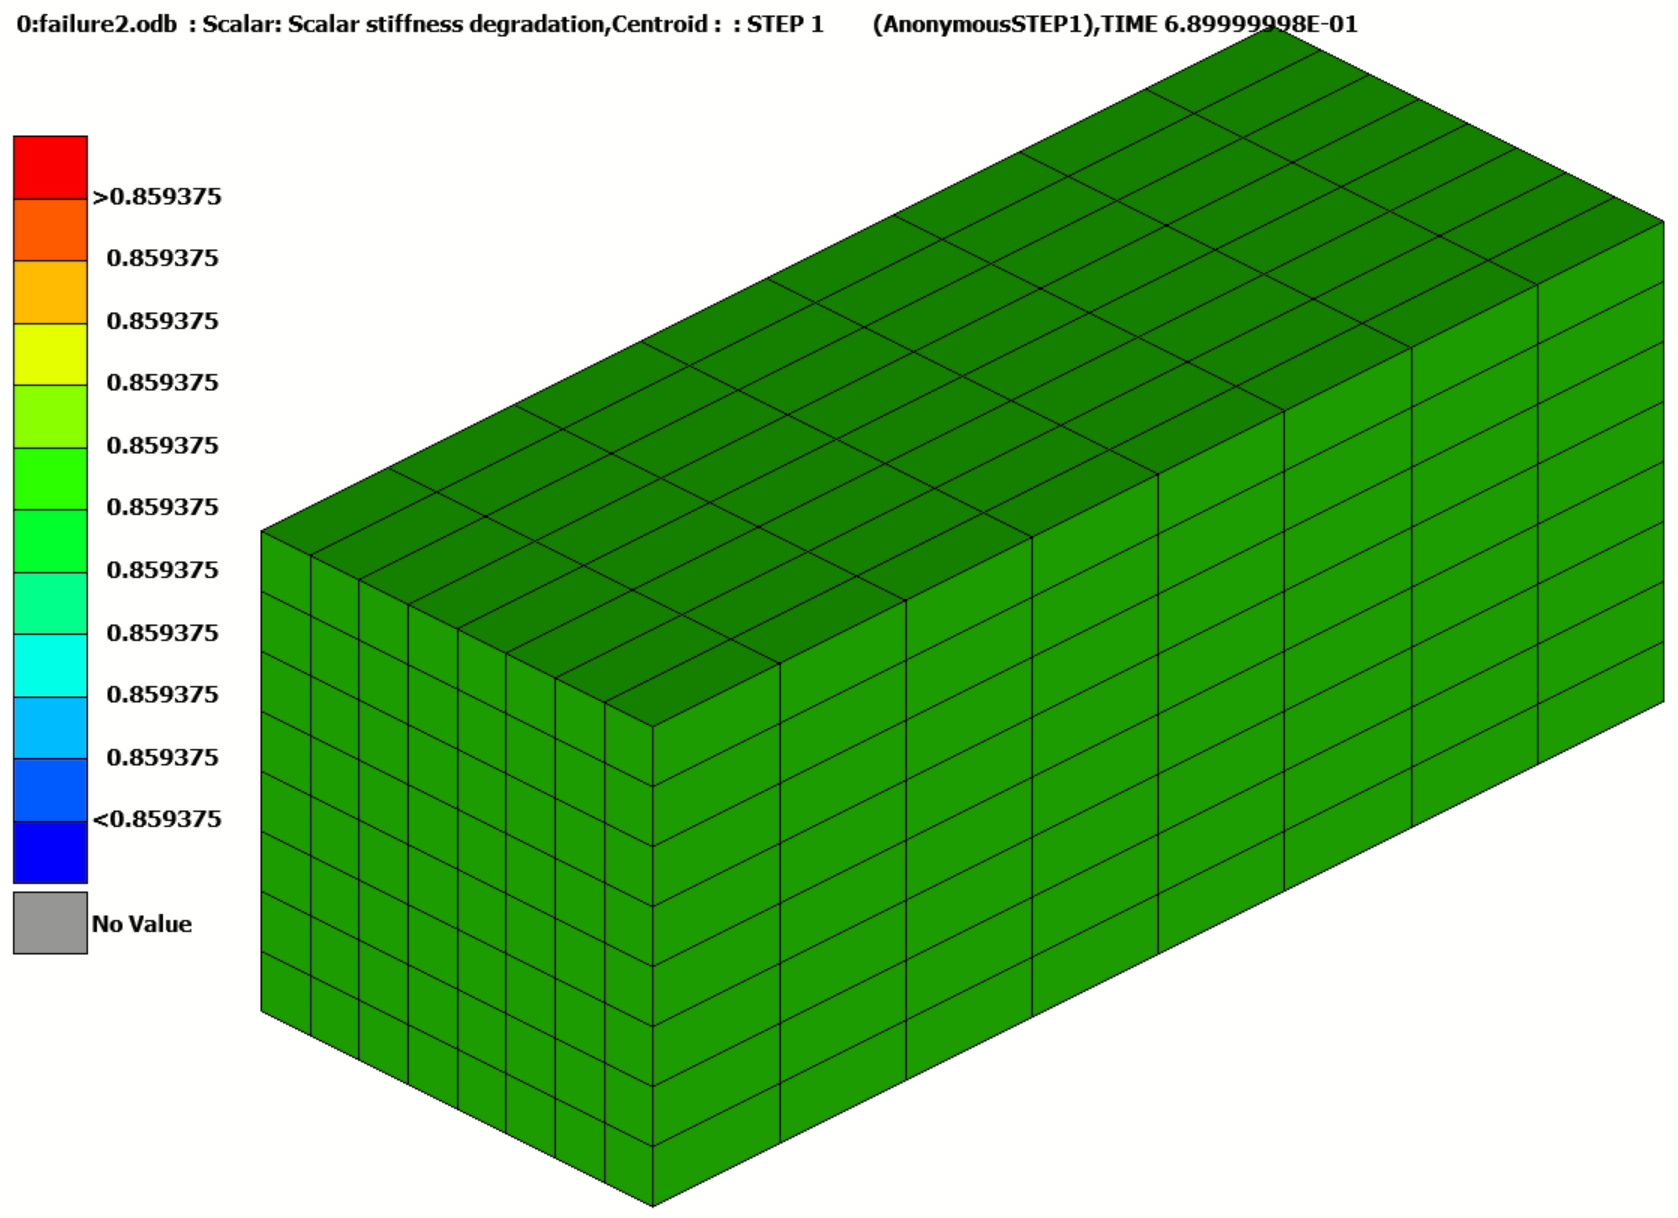
\includegraphics[width=\linewidth]{media/sdeg1.png}
        \caption{Βήμα επίλυσης 70.}
        \label{fig:label1}
    \end{subfigure}
    \hfill
    \begin{subfigure}{0.3\linewidth}
        \centering
        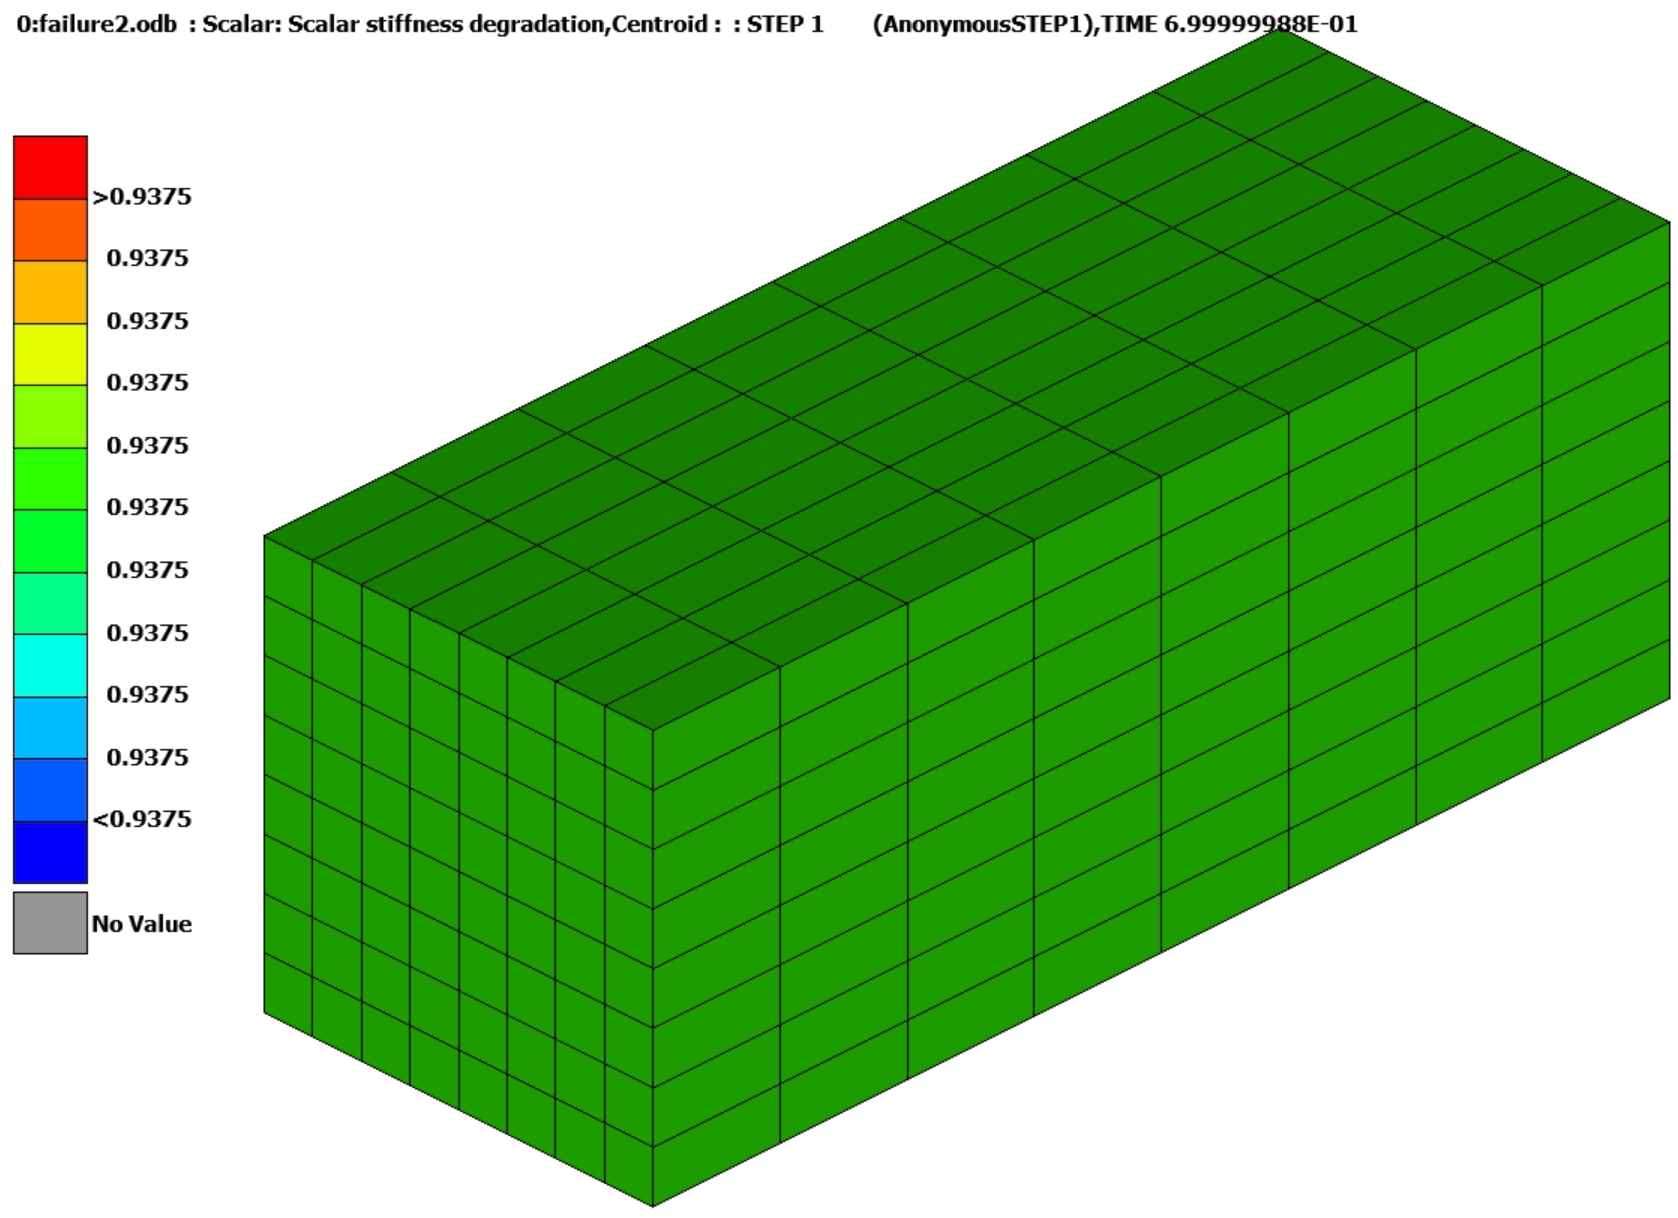
\includegraphics[width=\linewidth]{media/sdeg2.png}
        \caption{Βήμα επίλυσης 71.}
        \label{fig:label2}
    \end{subfigure}
    \hfill
    \begin{subfigure}{0.3\linewidth}
        \centering
        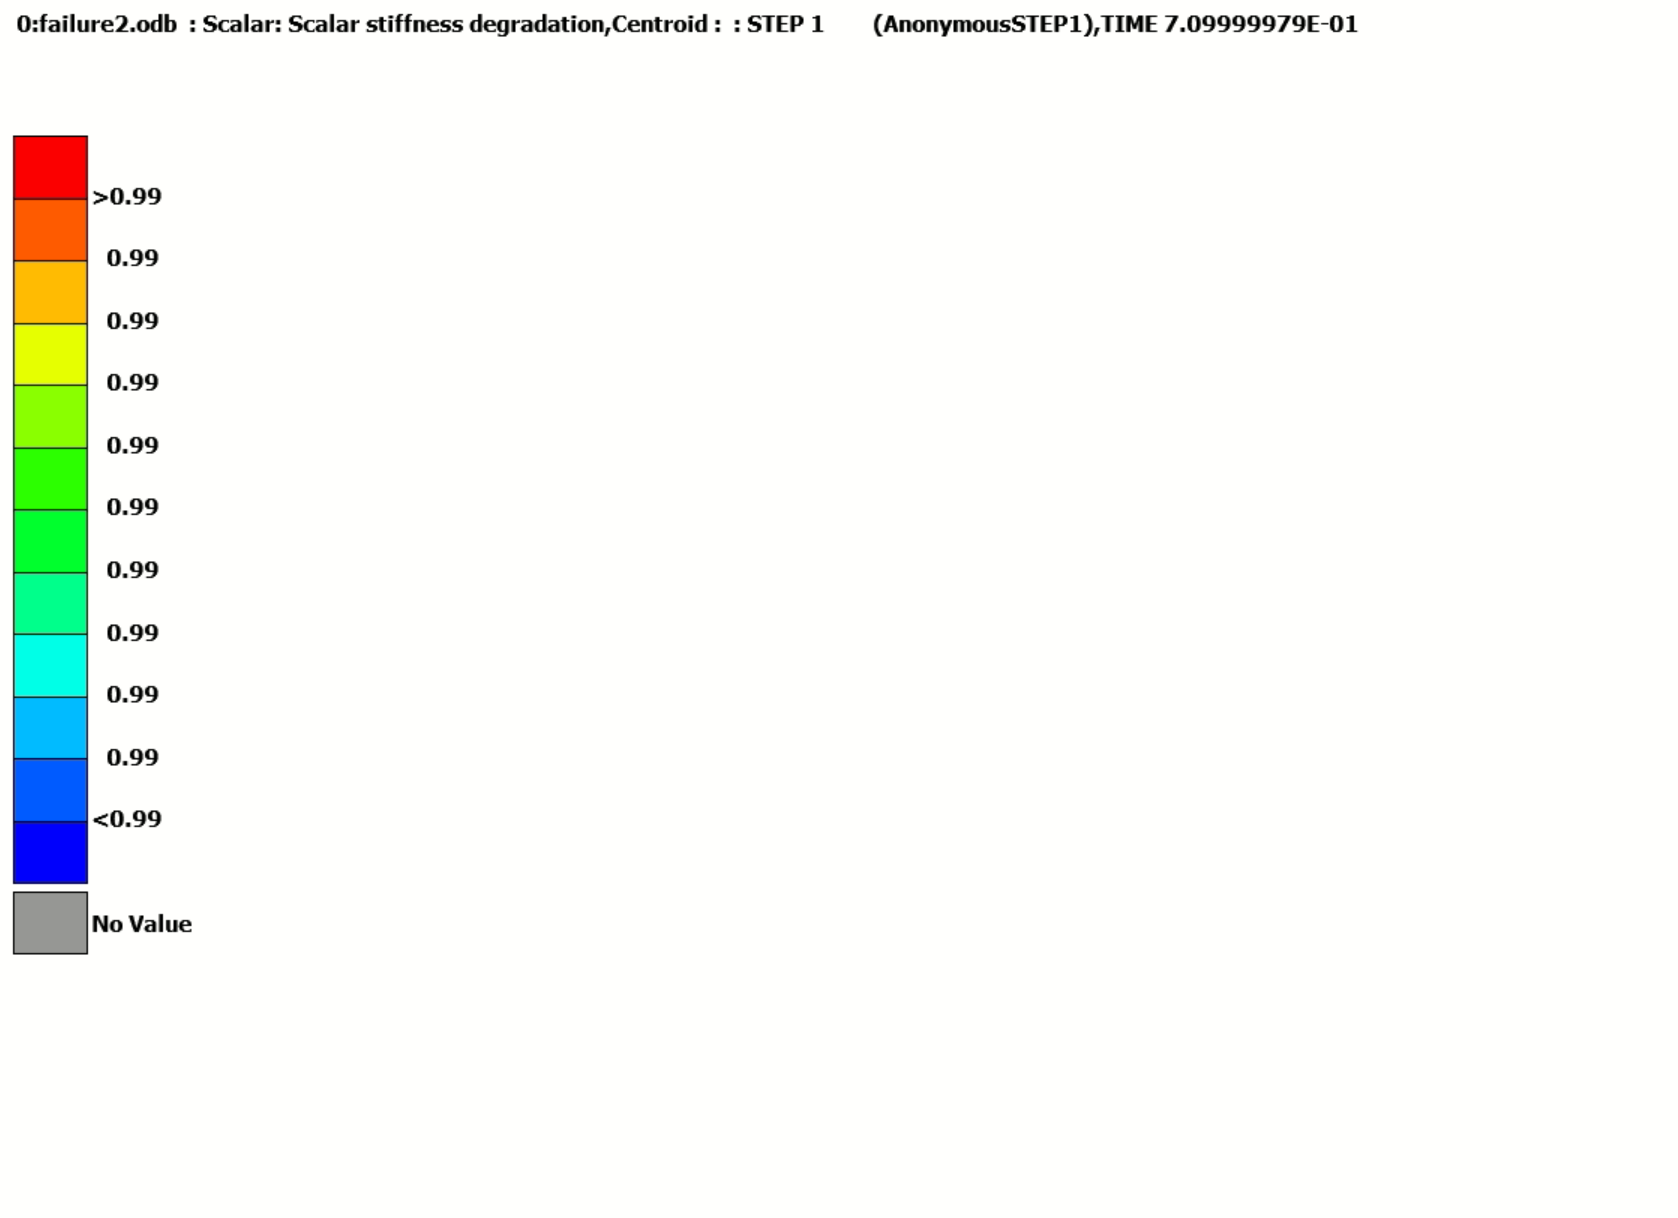
\includegraphics[width=\linewidth]{media/sdeg3.png}
        \caption{Βήμα επίλυσης 72.}
        \label{fig:label3}
    \end{subfigure}
    \caption{Διαγραφή στοιχείων μέγιστης υποβάθμισης.}
    \label{fig:steps}
\end{figure}

\begin{figure}[H]
    \centering
    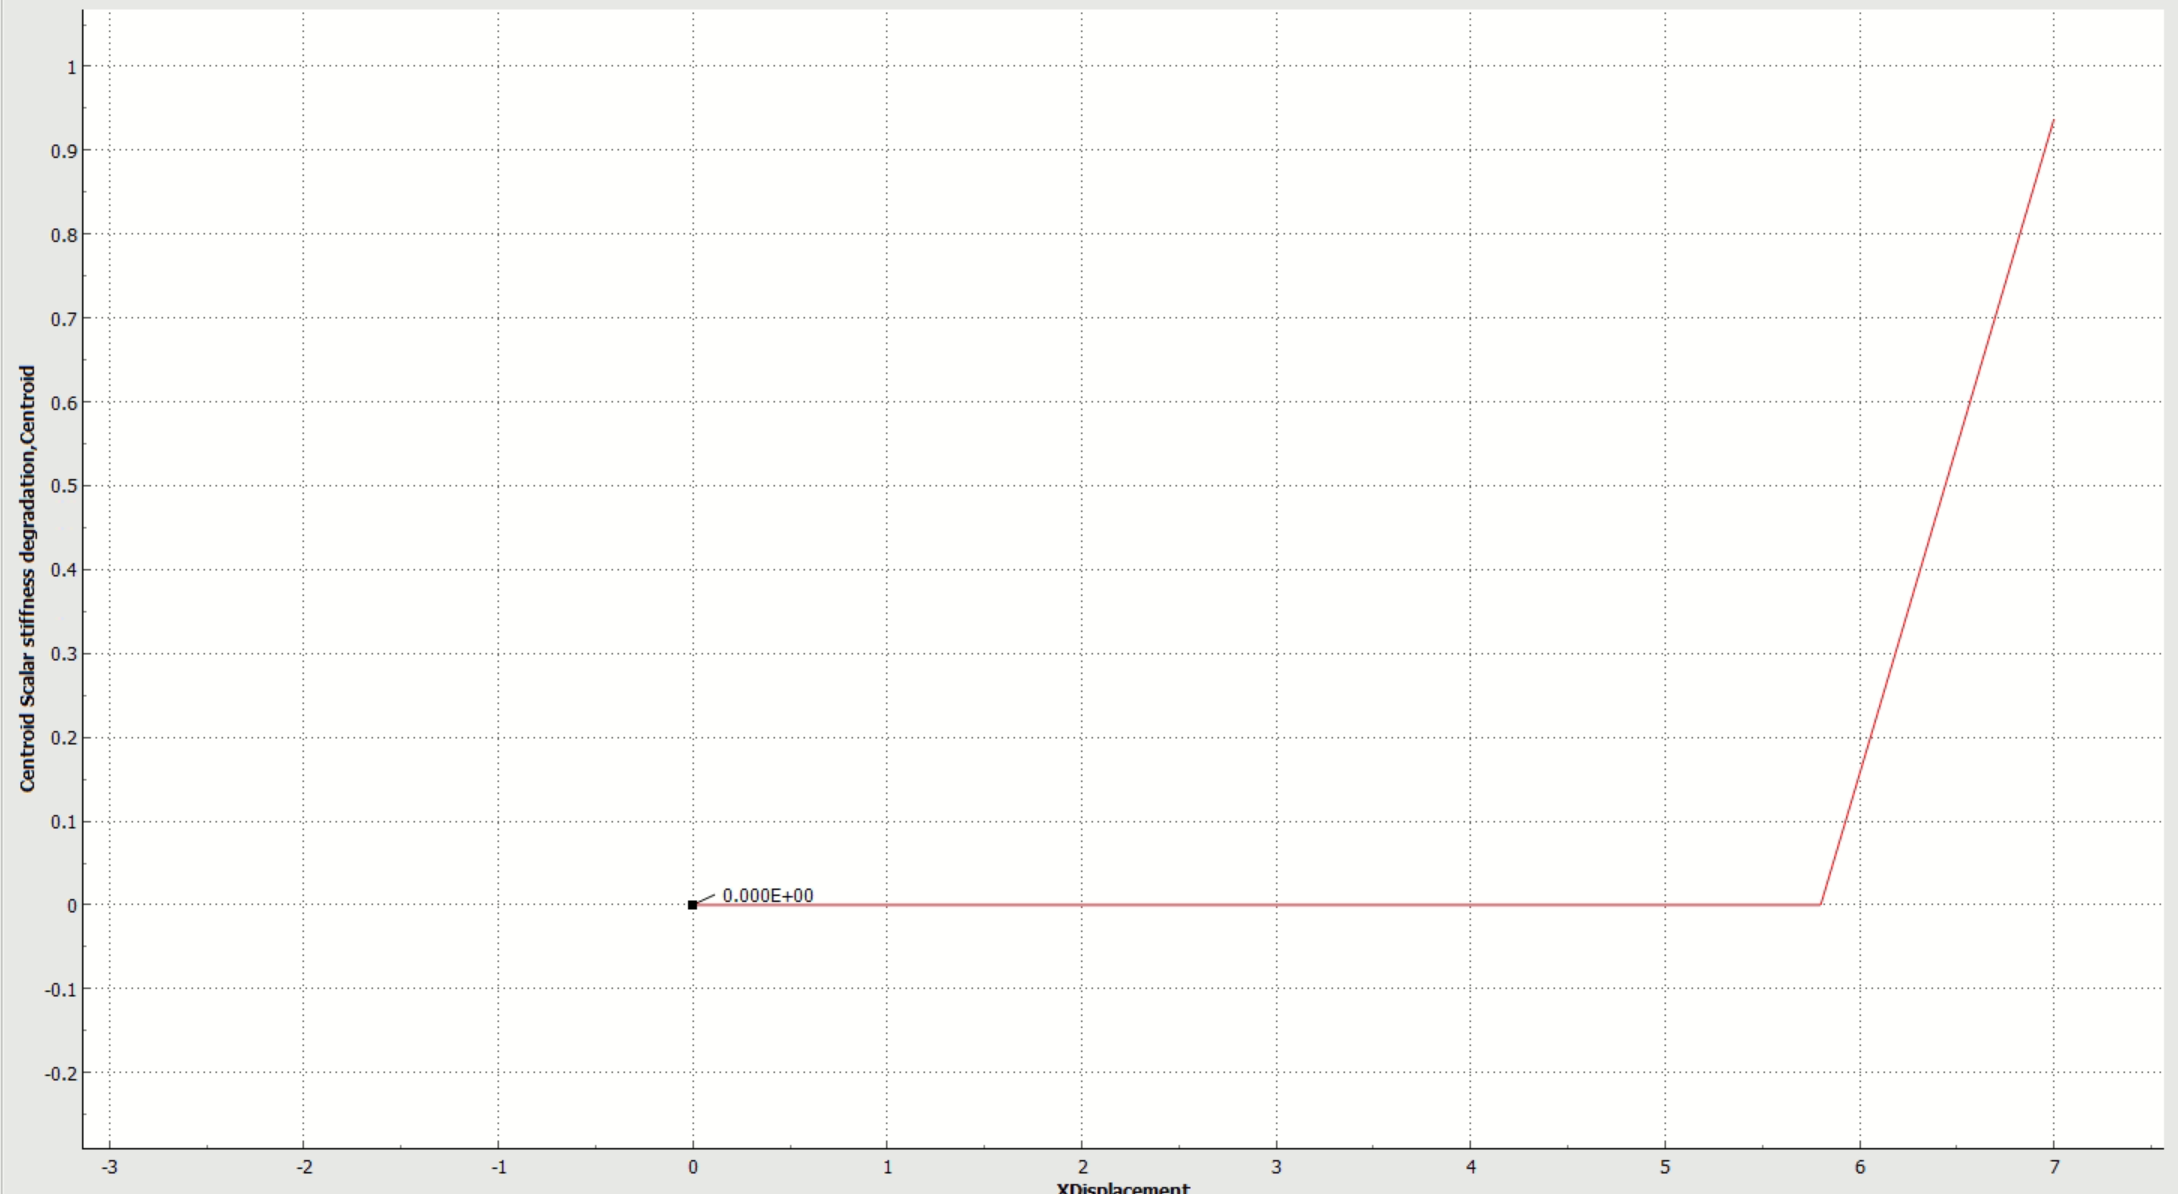
\includegraphics[width=0.7\linewidth]{media/sdeg-u.png}
    \caption{Εξέλιξη βλάβης με τη μετατόπιση.}
    \label{fig:sdegu}
\end{figure}


\subsection{Συμπεράσματα}











\listoffigures
\listoftables

\nocite{*}
\printbibliography

\end{document}